% Figure environments and captions for the manuscript (Phase 8 guidance, section 8 item 3).
%
% Captions are moved here from paper/FIGURE_CAPTIONS_DRAFT.md; tests/test_paper_assets.py checks that every number in
% this file also appears in that reviewed draft. Each PDF is drawn at its printed width (15 cm), so include it at its
% natural size: do not add width= or scale=, or the 8-12 pt text rule no longer holds. Place each figure near its
% first citation; the journal numbers figures in citation order. Panel letters are inside the images; captions are not.
% Paths are relative to paper/ (the manuscript root holds a figures/ folder). Labels match the results draft. All data come from classical simulation; none is from quantum hardware.

\begin{figure}[t]
  \centering
  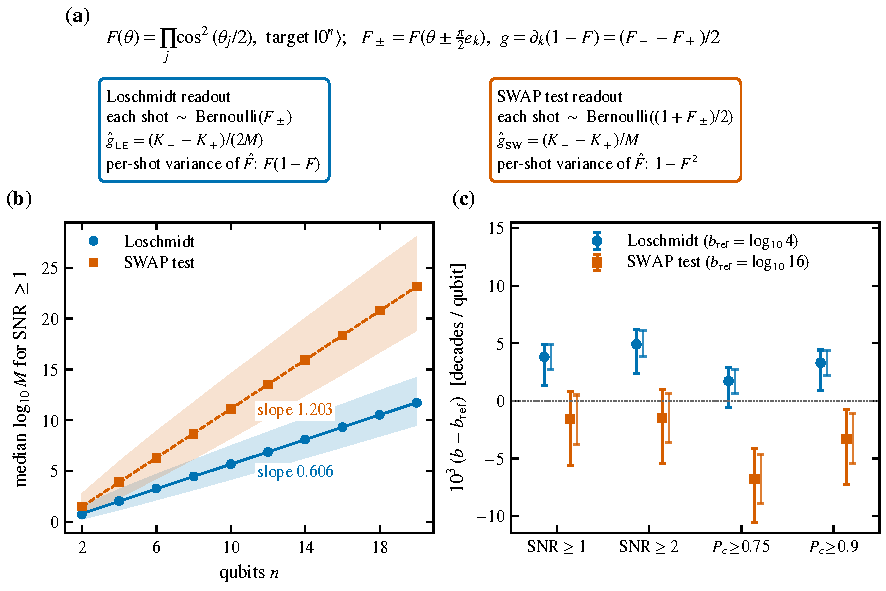
\includegraphics{figures/fig1_same_landscape.pdf}
  \caption{One landscape, two readouts.
    (a)~The Stage~7 benchmark: an RX product state on $n$ qubits with target $|0^n\rangle$ and fidelity
    $F(\theta) = \prod_j \cos^2(\theta_j/2)$, $\theta_j \sim U[-\pi, \pi]$, and the parameter-shift gradient of
    $C = 1 - F$ with respect to $\theta_k$ ($k = 0$). The two shifted fidelities are estimated either by a Loschmidt
    (projector) readout or by an ancilla SWAP test. Both readouts estimate the same $F_\pm$ and the same exact gradient
    $g$; they differ only in the per-shot statistics, $F(1 - F)$ for Loschmidt and $1 - F^2$ for SWAP.
    % (a) is a placeholder until the Figure 1(a) schematic (Shravan, due 19 Nov) replaces it.
    (b)~Median $\log_{10}$ of the shots per shifted circuit, $M$, needed for SNR $\ge 1$, over 100,000 $\theta$ per $n$,
    $n = 2$--$20$, the same $\theta$ for both readouts. Shaded bands are the interquartile range over $\theta$. Lines are
    the committed least-squares fits: slope 0.606 (Loschmidt) and 1.203 (SWAP) decades per qubit, close to
    $\log_{10} 4$ and $\log_{10} 16$.
    (c)~For four targets (SNR $\ge 1$, SNR $\ge 2$, sign accuracy $P_c \ge 0.75$ and $P_c \ge 0.9$), the Stage~7 slope
    minus its reference ($\log_{10} 4$ for Loschmidt, $\log_{10} 16$ for SWAP), in units of $10^{-3}$ decades per qubit.
    Thick bars: 95\% percentile interval over 20 independent seeds of 25,000 $\theta$ (B3). Thin bars: the B3
    $\theta$-bootstrap 95\% CI.
    The bases $4^n$ and $16^n$ belong to this RX-product benchmark, where the median shifted-fidelity sum decays as
    $4^{-n}$; they are not universal, and other circuits have other base rates (figure~\ref{fig:b1}). Only one parameter
    position ($k = 0$) and noiseless circuits are shown.}
  \label{fig:landscape}
\end{figure}

\begin{figure}[t]
  \centering
  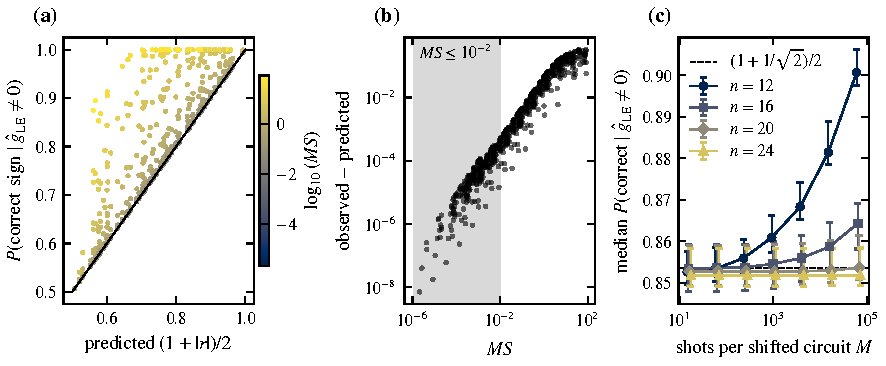
\includegraphics{figures/fig2_conditional_sign_law.pdf}
  \caption{Conditional sign accuracy of the Loschmidt gradient.
    (a)~The exact probability that a nonzero Loschmidt gradient estimate has the correct sign, against the prediction
    $(1 + |r|)/2$, where $r = (F_- - F_+)/(F_- + F_+)$. The 720 points cover the 16 B1 entangling cells at $n = 12$,
    $\theta$ at five quantiles of $S = F_+ + F_-$, and $M = 1$ to 65,536 shots per shifted circuit. Colour is
    $\log_{10}(MS)$.
    (b)~Observed minus predicted, against $MS$. It is positive in every row and falls with $MS$. For $MS \le 10^{-2}$
    (shaded) the largest deviation is $4.8 \times 10^{-4}$.
    (c)~The median over $\theta$ of the same probability on the regenerated Stage~7 RX-product population, computed
    without cancellation (B3), for $n = 12$--$24$ and $M = 16$--65,536. Error bars: 95\% percentile interval over 20
    seeds. Dashed line: $(1 + 1/\sqrt{2})/2 = 0.8536$, the population median of the prediction. At $n = 20$ and the
    Stage~7 shot counts ($M = 64$, 1,024 and 16,384) the median is 0.8527--0.8530.
    The prediction is a limit for $MS \to 0$. Departures at large $MS$, visible at $n = 12$ for $M \ge 1{,}024$, are
    expected and are not refitted. Panel (a) is exact (no sampling).}
  \label{fig:sign}
\end{figure}

\begin{figure}[t]
  \centering
  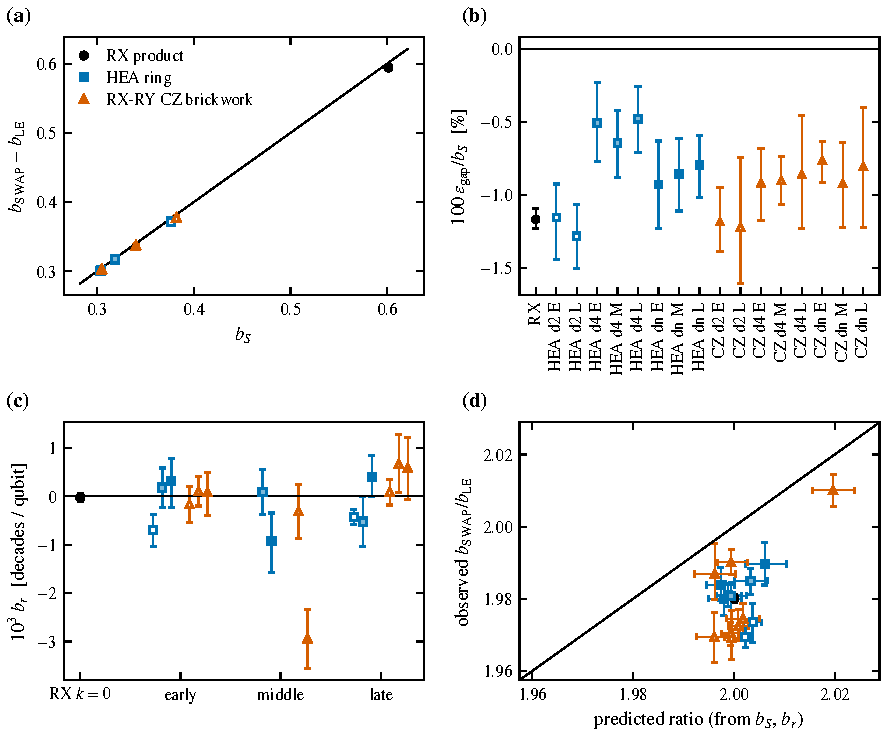
\includegraphics{figures/fig3_b1_scaling_rule.pdf}
  \caption{The slope rule across entangling circuits (B1). Slopes of median $\log_{10}$ quantities against $n$ for 17
    cells: the RX-product regression arm ($n = 2$--$20$); a hardware-efficient ring ansatz (RY, RZ, CNOT ring); and an
    RX-RY CZ brickwork ansatz. The two entangling ansätze are run at depth 2, depth 4 and depth $n$, with the
    differentiated parameter in the early, middle or late layer, on $n = 4$--16 (depth 2 and 4) or $n = 4$--14
    (depth $n$). Each cell uses 10 seeds of 4,000 $\theta$ per $n$. Marker shape and colour give the family; marker fill
    gives the depth (hollow: 2, half: 4, filled: $n$). Error bars are bootstrap 95\% CIs of the 10-seed mean.
    (a)~The measured gap $b_{\rm SWAP} - b_{\rm LE}$ against $b_S$, the slope of the shifted-fidelity sum; the line is
    equality.
    (b)~The residual $\varepsilon_{\rm gap} = (b_{\rm SWAP} - b_{\rm LE}) - b_S$ as a percentage of $b_S$. It ranges
    from $-1.28\%$ to $-0.48\%$.
    (c)~$b_r$, the slope of the relative gradient $|r|$, by parameter position. Every $|b_r| \le 3 \times 10^{-3}$
    decades per qubit. Six cells have CIs that exclude zero; the largest is the brickwork depth-$n$ middle cell
    ($-2.9 \times 10^{-3}$).
    (d)~The observed exponent ratio $b_{\rm SWAP}/b_{\rm LE}$ against the ratio predicted from the same cell's $b_S$
    and $b_r$. The observed ratios (1.969--2.010) lie 0.5--1.6\% below the prediction.
    Two ansatz families, one target state, noiseless circuits and $n \le 16$. The sub-percent residual is reported,
    not removed.}
  \label{fig:b1}
\end{figure}

\begin{figure}[t]
  \centering
  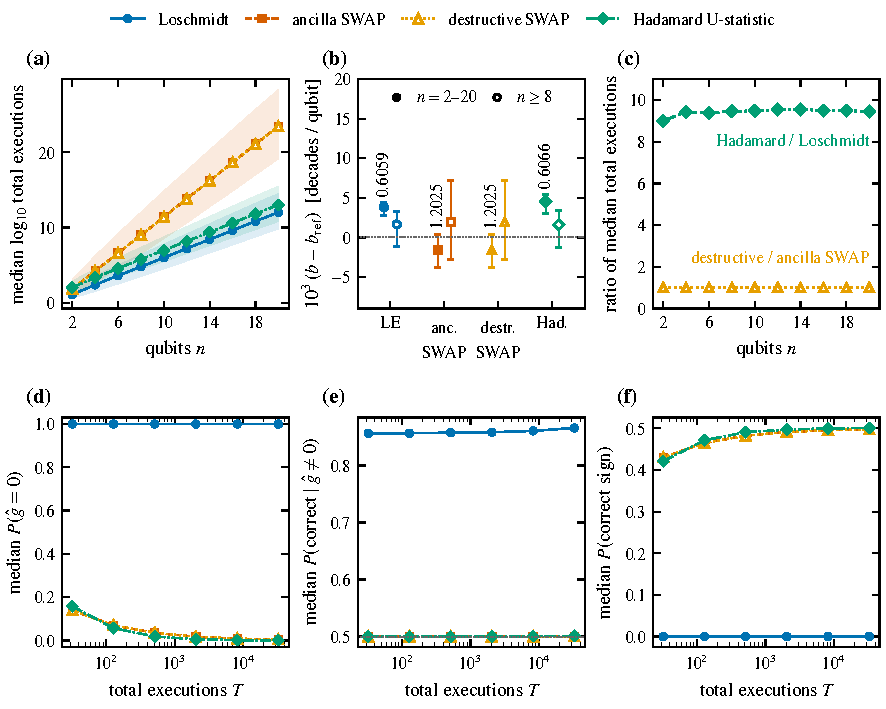
\includegraphics{figures/fig4_four_estimators.pdf}
  \caption{Four fidelity-gradient estimators on the RX-product landscape (B2): Loschmidt, ancilla SWAP, destructive
    SWAP (two copies, no ancilla) and a Hadamard-test U-statistic.
    (a)~Median $\log_{10}$ total circuit executions per gradient component for SNR $\ge 1$, on the Stage~7 population of
    100,000 $\theta$ per $n$, $n = 2$--$20$. Bands are interquartile ranges. The destructive and ancilla SWAP medians
    agree to $2 \times 10^{-13}$.
    (b)~Each fitted slope minus its reference ($\log_{10} 4$ for Loschmidt and Hadamard, $\log_{10} 16$ for the SWAPs),
    in $10^{-3}$ decades per qubit, for $n = 2$--$20$ (filled) and $n \ge 8$ (open). Error bars are 95\% percentile
    intervals over 10 replicate seeds of 25,000 $\theta$. Printed values are the $n = 2$--$20$ slopes.
    (c)~Ratio of median total executions: Hadamard to Loschmidt is 9.0 at $n = 2$ and 9.4--9.55 for $n \ge 4$;
    destructive to ancilla SWAP is 1.
    (d--f)~At $n = 14$ and a fixed budget of $T$ total executions: (d)~the median probability of an exactly zero
    estimate; (e)~the median probability of the correct sign given a nonzero estimate; (f)~the median probability of
    the correct sign. These are exact enumerations, except Hadamard at $T \ge 8{,}192$, which is Monte Carlo with
    20,000 repetitions.
    Executions are counted per gradient component. Qubit number, circuit depth, ancillas and the number of state copies
    differ between readouts, so equal execution counts do not mean equal hardware cost. Noiseless simulation only.}
  \label{fig:estimators}
\end{figure}

\begin{figure}[t]
  \centering
  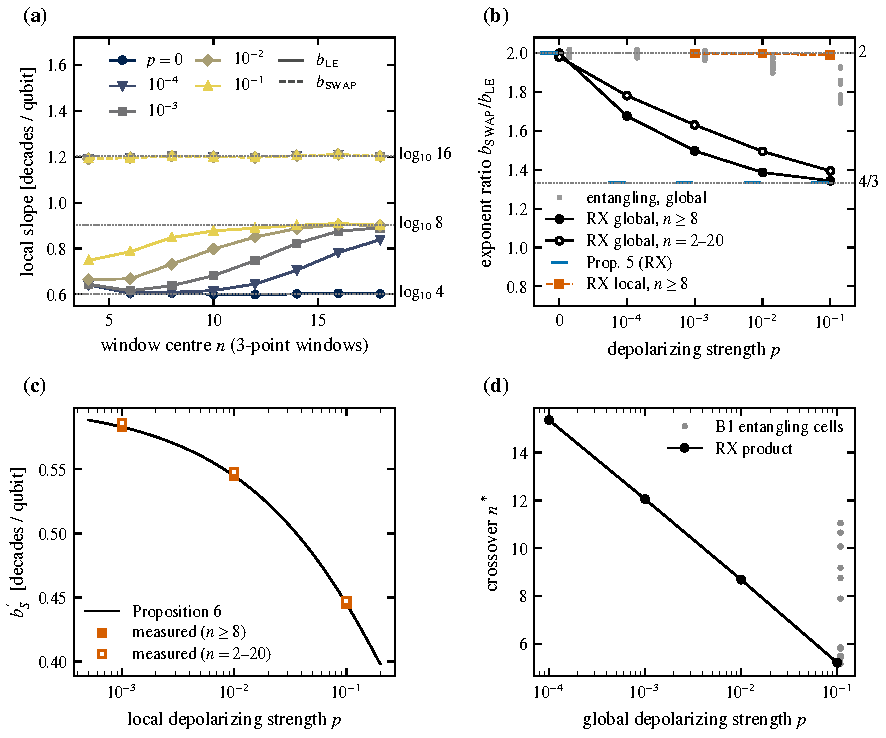
\includegraphics{figures/fig5_noise.pdf}
  \caption{Depolarizing noise (B4). Global depolarizing noise acts after every layer, which is exactly equivalent to
    $F' = qF + (1 - q)/2^n$ with $q = (1 - p)^L$. It is applied to the RX product ($L = 1$) and to the 16 B1 entangling
    cells. Local single-qubit depolarizing noise is applied to the RX product only. The data reuse the B1 $\theta$
    populations (10 seeds).
    (a)~Three-point local slopes of the seed-mean medians for the RX product under global noise: Loschmidt
    $b_{\rm LE}$ (filled markers, solid lines) and SWAP $b_{\rm SWAP}$ (open markers, dashed lines), for $p = 0$ to
    $10^{-1}$; marker shape and colour give $p$. With noise, $b_{\rm LE}$ rises from $\log_{10} 4$ toward $\log_{10} 8$
    (0.90 at the largest window for $p \ge 10^{-2}$). $b_{\rm SWAP}$ stays at 1.20.
    (b)~$b_{\rm SWAP}/b_{\rm LE}$ against $p$: the RX product under global noise, fitted over $n = 2$--$20$ (open) and
    $n \ge 8$ (filled); the committed Proposition~5 asymptote for the RX product (bars); the RX product under local
    noise (squares); and the 16 entangling cells under global noise (gray, $n \ge 8$).
    (c)~Measured $b_S'$ for the RX product under local noise, with the closed form of Proposition~6 (line).
    (d)~The crossover $n^*$, where the noise floor equals the noiseless signal scale, for the RX product ($n^* = 15.4$,
    12.1, 8.7 and 5.2 at $p = 10^{-4}$ to $10^{-1}$) and for the 13 entangling cells whose crossover lies inside the
    tested range (all at $p = 10^{-1}$). Cells where the signal dominates throughout are not plotted.
    Simulated depolarizing channels only, with an ideal SWAP target copy. Other noise channels, local noise on
    entangling circuits, and hardware are not covered. The fixed-depth entangling cells are mostly pre-asymptotic at
    $n \le 16$.}
  \label{fig:noise}
\end{figure}

\begin{figure}[t]
  \centering
  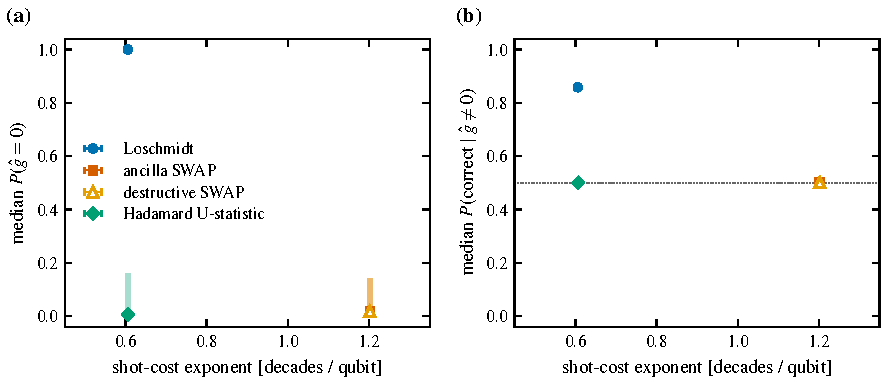
\includegraphics{figures/fig6_empirical_estimator_comparison.pdf}
  \caption{Empirical estimator comparison (not a theorem or a complete taxonomy). For the four estimators of
    figure~\ref{fig:estimators}, the horizontal axis is the fitted shot-cost exponent (median total executions,
    $n = 2$--$20$, with the 95\% replicate interval). The vertical axis is a finite-shot failure statistic for the RX
    product at $n = 14$: (a)~the median probability of an exactly zero estimate; (b)~the median probability of the
    correct sign given a nonzero estimate. Markers are the values at $T = 2{,}048$ total executions; the shaded bars
    show the range over $T = 32$--32,768. Loschmidt combines the lower exponent with exact-zero estimates. Both SWAP
    readouts combine the higher exponent with nonzero estimates whose sign is correct half the time. The Hadamard
    U-statistic combines the lower exponent with nonzero estimates whose sign is correct half the time.
    One landscape (RX product), one $n$ and the B2 budget grid. Whether exponent and failure type are independent
    properties in general is an open question (P4); this figure shows measured values only.}
  \label{fig:failure}
\end{figure}

% ---------------------------------------------------------------------------------------------------------------------
% SLOT: failure-type grid. Goes in only if P4 (the failure-type lemma, Satyabrat with Shravan, due 18 Nov) succeeds.
% If it does, it becomes the organising figure for Main 3 and is cited early, so the numbering above shifts (the
% journal numbers figures in citation order). If P4 fails, Main 3 is an empirical observation and figure~\ref{fig:failure}
% above is its only figure. Build it in src/qlo/paper/figures.py like the others (15 cm wide, 8-12 pt, sources listed).
%
% \begin{figure}[t]
%   \centering
%   \includegraphics{figures/fig7_failure_type_grid.pdf}
%   \caption{Failure-type grid. ...}
%   \label{fig:failure-grid}
% \end{figure}
